\section{Image processing: Earth Observation - Medical imaging - Astronomy}

\begin{frame}{Earth Observation - Medical - Astronomy}

  \begin{block}{Common ground}
    \begin{itemize}
    \item We all process complex and large datasets
    \item We produce images that experts should interpret
    \item Different applications but some common methods and algorithms
    \end{itemize}
  \end{block}

  \begin{block}{Don't reinvent the wheel}
    \begin{itemize}
    \item OTB architecture is based on the medical image processing library ITK
    \item Reuse other specific libraries (machine learning\ldots)
    \item Generic libraries $\rightarrow$ extend the use of the tool  
    \item Example of usage of ITK/OTB in other contexts 
    \item Can work the other way around
    \end{itemize}
  \end{block}

\end{frame}

\begin{frame}{VAHINE: Visualization and analysis of multi-dimensional
    hyperspectral images in Astrophysics (Planétologie Grenoble)}
  \begin{center}
    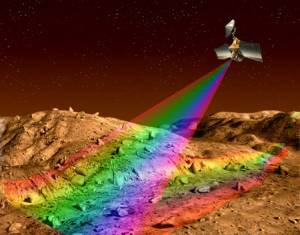
\includegraphics[keepaspectratio,height=0.6\paperheight]{images/crism-mars.jpg}
  \end{center}  
\end{frame}

\begin{frame}{GUI for visualizing and processing (OTB+QGIS)}
  \begin{center}
    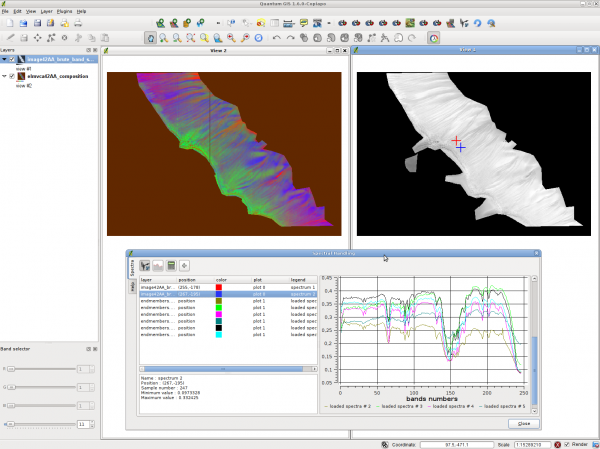
\includegraphics[keepaspectratio,height=0.6\paperheight]{images/vahine-qgis.png}
  \end{center}  
\end{frame}

\begin{frame}{Visualization of astronomical data in ITK/Slicer (star forming
    region IC 348) - Astromed project - ICC Harvard}
  \centering
    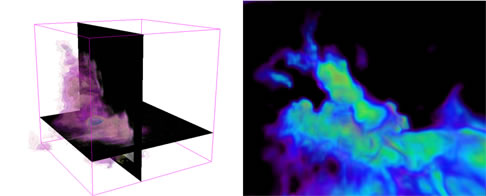
\includegraphics[height=0.6\paperheight]{images/Astromed1-mj.jpg}
\end{frame}
